
The character classifier classifies images that contain handwritten characters, as described in Section~\ref{sec:overview-of-classifiers}. 
%% Sorry I don't really get what you want to say with this sentence, I changed based on what I think you mean, but it should probably be changed again -- Fabian
A sequence of observation symbols is extracted from the supplied training data and used when an image is to be classified. 
This process is called feature extraction. 

    \begin{figure}[htb] 
      \begin{center}
	\leavevmode
	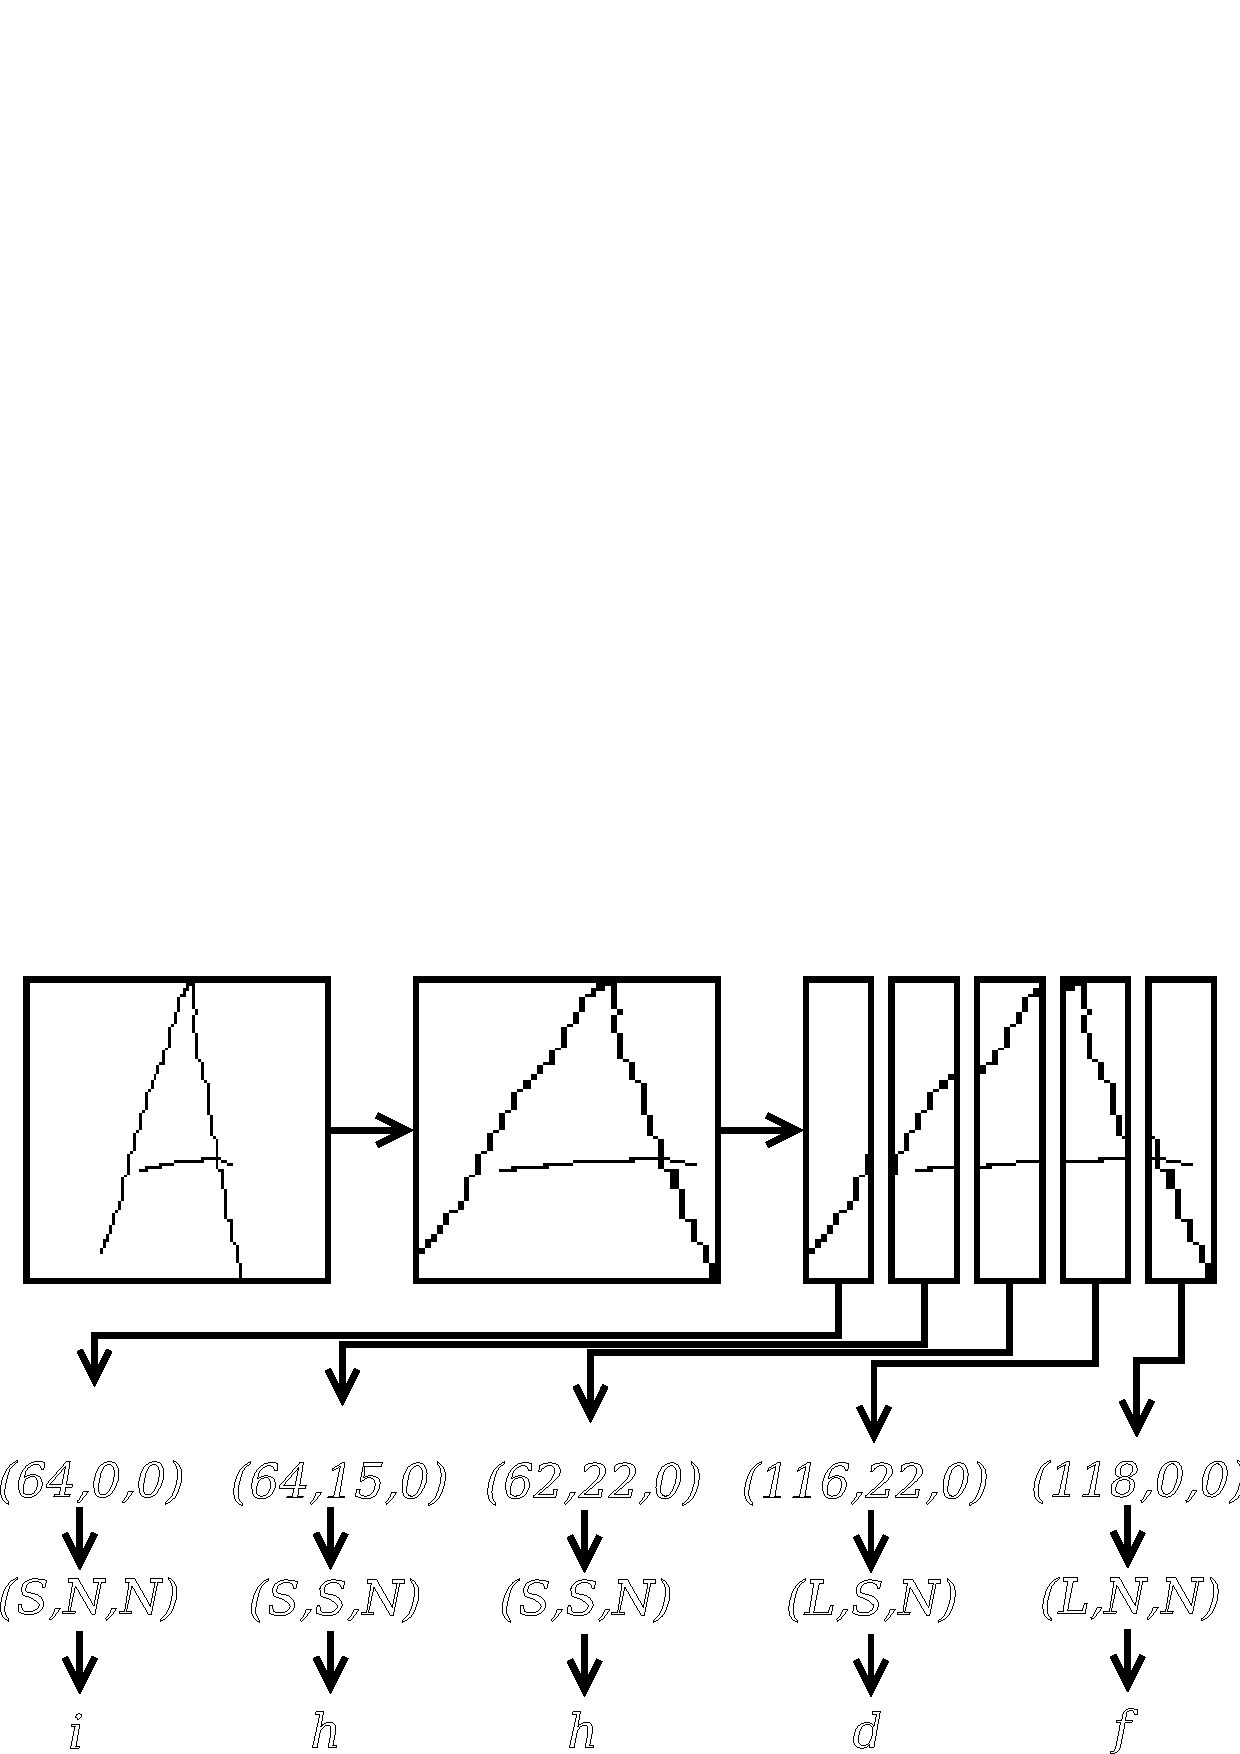
\includegraphics[width=110mm]{image_feature_extraction.pdf}%width=115mm,height=40mm
      \end{center}
      \caption{An illustration of the feature extraction process.}
      \label{fig:image_feature_extraction}
    \end{figure}


As mentioned in Section~\ref{sec:introduction}, our system assumes that there is one image per character, that the lines in the characters consists of a single color and that the lines are one pixel wide. The feature extraction process can be divided into the following steps:

\begin{enumerate}
  \item The scaling step makes sure that the character fills the whole image. 
  Because of this step, it does not matter where in the given image the character is painted. 
  The scaling may cause a problem because the lines may get thicker than one pixel after scaling, if the original painted character just fills a small part of the image\footnote{The standard Java image scaling algorithm is used for the scaling.}. 
  %% Shouldn't the following sentence be 'a large part' ??? -- Fabian
  This problem will be avoided if the training examples contain images where the character fills a small part of the image.
  This is because the model will learn to recognize images with thicker lines.
  The following algorithm is used to do the scaling:
  \begin{enumerate}
    \item The minimum rectangle $R$ in the image that contains the whole character is found.
    \item The rectangle $R$ is scaled to fill the size of the original image. 
    The scaled version of $R$ is returned as the scaled image.
  \end{enumerate}
  \item The new scaled image is sliced into $N$ vertical segments of the same size.
  \item An observation symbol is extracted from every segment in the following way:
  \begin{enumerate}
    \item The number of pixels in the three largest components in the segment are found. 
    The component sizes are then put into a triple $(s_{1},s_{2},s_{3})$ that is sorted so that the largest number is first. 
    A component is defined as a set of colored pixels that are connected and that contains all pixels that are connected to one of the pixels in the set. 
    Two colored pixels are connected if they are neighbors or if it is possible to create a path of colored connected pixels between them. 
    All pixels except the border pixels have 8 neighbors. 
    If the segment contains less than three components, the triple is filled with zeros. 
    
    So for example if a segment contains two lines. 
    One line containing 10 pixels and another line containing 5 pixels. 
    Then the resulting triple will be $(10,5,0)$.
    \item The elements in the triple is classified as $Large$, $Small$ or $None$. 
    The classification function $c$ is defined as in Equation~\ref{eq:classification_function}. 
    The constant $d$ in the equation is given as a parameter to the feature extraction.
    \begin{equation}\label{eq:classification_function}
    c(s) = None \text{ if } s = 0, Large \text{ if } s > d \text{ and } Small \text{ otherwise}.
    \end{equation}
    The triple $(s_{1},s_{2},s_{3})$ is translated to a triple of classes $(c_{1},c_{2},c_{3})$ by applying the function $c$ to all elements in the triple.
    \item The triple of classes is mapped to an observation symbol.
    In total there are 10 different triples and there is one observation symbol per triple. 
    So in total there are 10 different observation symbols. 
%The mapping is defined by the set of relations that can be found in Equation~\ref{eq:class_triple_to_observation_symbol_mappings}.
    %\begin{equation}\label{eq:class_triple_to_observation_symbol_mappings}
    % \substack{ LLL\rightarrow a,LLS\rightarrow b,LSS\rightarrow c,LSN\rightarrow d,LLN\rightarrow e,LNN\rightarrow f,\\
    %SSS\rightarrow g,SSN\rightarrow h,SNN\rightarrow i,NNN,\rightarrow j }
    %\end{equation}
    %% This looks weird imo.
     %$LSN$ is a short form of $(Large,Small,None)$ and so on.
  \end{enumerate}  
\end{enumerate}

The classification constant $d$ and the number of segments $N$ are parameters to the feature extractor. 
An example of feature extraction for an image can be seen in Figure~\ref{fig:image_feature_extraction}.